\documentclass[1p]{elsarticle_modified}
%\bibliographystyle{elsarticle-num}

%\usepackage[colorlinks]{hyperref}
%\usepackage{abbrmath_seonhwa} %\Abb, \Ascr, \Acal ,\Abf, \Afrak
\usepackage{amsfonts}
\usepackage{amssymb}
\usepackage{amsmath}
\usepackage{amsthm}
\usepackage{scalefnt}
\usepackage{amsbsy}
\usepackage{kotex}
\usepackage{caption}
\usepackage{subfig}
\usepackage{color}
\usepackage{graphicx}
\usepackage{xcolor} %% white, black, red, green, blue, cyan, magenta, yellow
\usepackage{float}
\usepackage{setspace}
\usepackage{hyperref}

\usepackage{tikz}
\usetikzlibrary{arrows}

\usepackage{multirow}
\usepackage{array} % fixed length table
\usepackage{hhline}

%%%%%%%%%%%%%%%%%%%%%
\makeatletter
\renewcommand*\env@matrix[1][\arraystretch]{%
	\edef\arraystretch{#1}%
	\hskip -\arraycolsep
	\let\@ifnextchar\new@ifnextchar
	\array{*\c@MaxMatrixCols c}}
\makeatother %https://tex.stackexchange.com/questions/14071/how-can-i-increase-the-line-spacing-in-a-matrix
%%%%%%%%%%%%%%%

\usepackage[normalem]{ulem}

\newcommand{\msout}[1]{\ifmmode\text{\sout{\ensuremath{#1}}}\else\sout{#1}\fi}
%SOURCE: \msout is \stkout macro in https://tex.stackexchange.com/questions/20609/strikeout-in-math-mode

\newcommand{\cancel}[1]{
	\ifmmode
	{\color{red}\msout{#1}}
	\else
	{\color{red}\sout{#1}}
	\fi
}

\newcommand{\add}[1]{
	{\color{blue}\uwave{#1}}
}

\newcommand{\replace}[2]{
	\ifmmode
	{\color{red}\msout{#1}}{\color{blue}\uwave{#2}}
	\else
	{\color{red}\sout{#1}}{\color{blue}\uwave{#2}}
	\fi
}

\newcommand{\Sol}{\mathcal{S}} %segment
\newcommand{\D}{D} %diagram
\newcommand{\A}{\mathcal{A}} %arc


%%%%%%%%%%%%%%%%%%%%%%%%%%%%%5 test

\def\sl{\operatorname{\textup{SL}}(2,\Cbb)}
\def\psl{\operatorname{\textup{PSL}}(2,\Cbb)}
\def\quan{\mkern 1mu \triangleright \mkern 1mu}

\theoremstyle{definition}
\newtheorem{thm}{Theorem}[section]
\newtheorem{prop}[thm]{Proposition}
\newtheorem{lem}[thm]{Lemma}
\newtheorem{ques}[thm]{Question}
\newtheorem{cor}[thm]{Corollary}
\newtheorem{defn}[thm]{Definition}
\newtheorem{exam}[thm]{Example}
\newtheorem{rmk}[thm]{Remark}
\newtheorem{alg}[thm]{Algorithm}

\newcommand{\I}{\sqrt{-1}}
\begin{document}

%\begin{frontmatter}
%
%\title{Boundary parabolic representations of knots up to 8 crossings}
%
%%% Group authors per affiliation:
%\author{Yunhi Cho} 
%\address{Department of Mathematics, University of Seoul, Seoul, Korea}
%\ead{yhcho@uos.ac.kr}
%
%
%\author{Seonhwa Kim} %\fnref{s_kim}}
%\address{Center for Geometry and Physics, Institute for Basic Science, Pohang, 37673, Korea}
%\ead{ryeona17@ibs.re.kr}
%
%\author{Hyuk Kim}
%\address{Department of Mathematical Sciences, Seoul National University, Seoul 08826, Korea}
%\ead{hyukkim@snu.ac.kr}
%
%\author{Seokbeom Yoon}
%\address{Department of Mathematical Sciences, Seoul National University, Seoul, 08826,  Korea}
%\ead{sbyoon15@snu.ac.kr}
%
%\begin{abstract}
%We find all boundary parabolic representation of knots up to 8 crossings.
%
%\end{abstract}
%\begin{keyword}
%    \MSC[2010] 57M25 
%\end{keyword}
%
%\end{frontmatter}

%\linenumbers
%\tableofcontents
%
\newcommand\colored[1]{\textcolor{white}{\rule[-0.35ex]{0.8em}{1.4ex}}\kern-0.8em\color{red} #1}%
%\newcommand\colored[1]{\textcolor{white}{ #1}\kern-2.17ex	\textcolor{white}{ #1}\kern-1.81ex	\textcolor{white}{ #1}\kern-2.15ex\color{red}#1	}

{\Large $\underline{12a_{0328}~(K12a_{0328})}$}

\setlength{\tabcolsep}{10pt}
\renewcommand{\arraystretch}{1.6}
\vspace{1cm}\begin{tabular}{m{100pt}>{\centering\arraybackslash}m{274pt}}
\multirow{5}{120pt}{
	\centering
	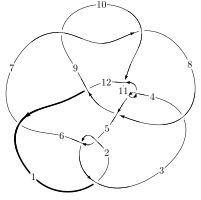
\includegraphics[width=112pt]{../../../GIT/diagram.site/Diagrams/png/1129_12a_0328.png}\\
\ \ \ A knot diagram\footnotemark}&
\allowdisplaybreaks
\textbf{Linearized knot diagam} \\
\cline{2-2}
 &
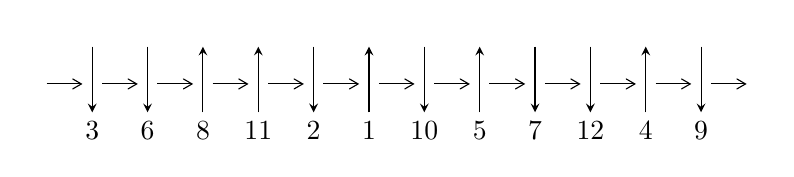
\begin{tikzpicture}[x=20pt, y=17pt]
	% nodes
	\node (C0) at (0, 0) {};
	\node (C1) at (1, 0) {};
	\node (C1U) at (1, +1) {};
	\node (C1D) at (1, -1) {3};

	\node (C2) at (2, 0) {};
	\node (C2U) at (2, +1) {};
	\node (C2D) at (2, -1) {6};

	\node (C3) at (3, 0) {};
	\node (C3U) at (3, +1) {};
	\node (C3D) at (3, -1) {8};

	\node (C4) at (4, 0) {};
	\node (C4U) at (4, +1) {};
	\node (C4D) at (4, -1) {11};

	\node (C5) at (5, 0) {};
	\node (C5U) at (5, +1) {};
	\node (C5D) at (5, -1) {2};

	\node (C6) at (6, 0) {};
	\node (C6U) at (6, +1) {};
	\node (C6D) at (6, -1) {1};

	\node (C7) at (7, 0) {};
	\node (C7U) at (7, +1) {};
	\node (C7D) at (7, -1) {10};

	\node (C8) at (8, 0) {};
	\node (C8U) at (8, +1) {};
	\node (C8D) at (8, -1) {5};

	\node (C9) at (9, 0) {};
	\node (C9U) at (9, +1) {};
	\node (C9D) at (9, -1) {7};

	\node (C10) at (10, 0) {};
	\node (C10U) at (10, +1) {};
	\node (C10D) at (10, -1) {12};

	\node (C11) at (11, 0) {};
	\node (C11U) at (11, +1) {};
	\node (C11D) at (11, -1) {4};

	\node (C12) at (12, 0) {};
	\node (C12U) at (12, +1) {};
	\node (C12D) at (12, -1) {9};
	\node (C13) at (13, 0) {};

	% arrows
	\draw[->,>={angle 60}]
	(C0) edge (C1) (C1) edge (C2) (C2) edge (C3) (C3) edge (C4) (C4) edge (C5) (C5) edge (C6) (C6) edge (C7) (C7) edge (C8) (C8) edge (C9) (C9) edge (C10) (C10) edge (C11) (C11) edge (C12) (C12) edge (C13) ;	\draw[->,>=stealth]
	(C1U) edge (C1D) (C2U) edge (C2D) (C3D) edge (C3U) (C4D) edge (C4U) (C5U) edge (C5D) (C6D) edge (C6U) (C7U) edge (C7D) (C8D) edge (C8U) (C9U) edge (C9D) (C10U) edge (C10D) (C11D) edge (C11U) (C12U) edge (C12D) ;
	\end{tikzpicture} \\
\hhline{~~} \\& 
\textbf{Solving Sequence} \\ \cline{2-2} 
 &
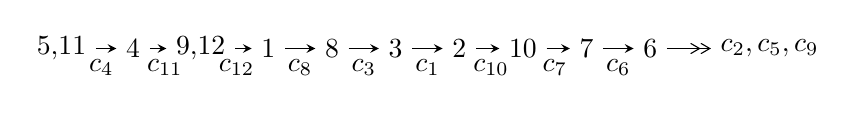
\begin{tikzpicture}[x=23pt, y=7pt]
	% node
	\node (A0) at (-1/8, 0) {5,11};
	\node (A1) at (1, 0) {4};
	\node (A2) at (33/16, 0) {9,12};
	\node (A3) at (25/8, 0) {1};
	\node (A4) at (33/8, 0) {8};
	\node (A5) at (41/8, 0) {3};
	\node (A6) at (49/8, 0) {2};
	\node (A7) at (57/8, 0) {10};
	\node (A8) at (65/8, 0) {7};
	\node (A9) at (73/8, 0) {6};
	\node (C1) at (1/2, -1) {$c_{4}$};
	\node (C2) at (3/2, -1) {$c_{11}$};
	\node (C3) at (21/8, -1) {$c_{12}$};
	\node (C4) at (29/8, -1) {$c_{8}$};
	\node (C5) at (37/8, -1) {$c_{3}$};
	\node (C6) at (45/8, -1) {$c_{1}$};
	\node (C7) at (53/8, -1) {$c_{10}$};
	\node (C8) at (61/8, -1) {$c_{7}$};
	\node (C9) at (69/8, -1) {$c_{6}$};
	\node (A10) at (11, 0) {$c_{2},c_{5},c_{9}$};

	% edge
	\draw[->,>=stealth]	
	(A0) edge (A1) (A1) edge (A2) (A2) edge (A3) (A3) edge (A4) (A4) edge (A5) (A5) edge (A6) (A6) edge (A7) (A7) edge (A8) (A8) edge (A9) ;
	\draw[->>,>={angle 60}]	
	(A9) edge (A10);
\end{tikzpicture} \\ 

\end{tabular} \\

\footnotetext{
The image of knot diagram is generated by the software ``\textbf{Draw programme}" developed by Andrew Bartholomew(\url{http://www.layer8.co.uk/maths/draw/index.htm\#Running-draw}), where we modified some parts for our purpose(\url{https://github.com/CATsTAILs/LinksPainter}).
}\phantom \\ \newline 
\centering \textbf{Ideals for irreducible components\footnotemark of $X_{\text{par}}$} 
 
\begin{align*}
I^u_{1}&=\langle 
1.70687\times10^{211} u^{118}+3.37461\times10^{211} u^{117}+\cdots+8.64942\times10^{211} b-9.37981\times10^{210},\\
\phantom{I^u_{1}}&\phantom{= \langle  }-7.88628\times10^{211} u^{118}-1.11014\times10^{212} u^{117}+\cdots+8.64942\times10^{211} a-7.17770\times10^{211},\\
\phantom{I^u_{1}}&\phantom{= \langle  }u^{119}+u^{118}+\cdots+6 u^3-1\rangle \\
\\
\end{align*}
\raggedright * 1 irreducible components of $\dim_{\mathbb{C}}=0$, with total 119 representations.\\
\footnotetext{All coefficients of polynomials are rational numbers. But the coefficients are sometimes approximated in decimal forms when there is not enough margin.}
\newpage
\renewcommand{\arraystretch}{1}
\centering \section*{I. $I^u_{1}= \langle 1.71\times10^{211} u^{118}+3.37\times10^{211} u^{117}+\cdots+8.65\times10^{211} b-9.38\times10^{210},\;-7.89\times10^{211} u^{118}-1.11\times10^{212} u^{117}+\cdots+8.65\times10^{211} a-7.18\times10^{211},\;u^{119}+u^{118}+\cdots+6 u^3-1 \rangle$}
\flushleft \textbf{(i) Arc colorings}\\
\begin{tabular}{m{7pt} m{180pt} m{7pt} m{180pt} }
\flushright $a_{5}=$&$\begin{pmatrix}1\\0\end{pmatrix}$ \\
\flushright $a_{11}=$&$\begin{pmatrix}0\\u\end{pmatrix}$ \\
\flushright $a_{4}=$&$\begin{pmatrix}1\\u^2\end{pmatrix}$ \\
\flushright $a_{9}=$&$\begin{pmatrix}0.911771 u^{118}+1.28348 u^{117}+\cdots+2.73608 u+0.829848\\-0.197340 u^{118}-0.390155 u^{117}+\cdots+3.02815 u+0.108444\end{pmatrix}$ \\
\flushright $a_{12}=$&$\begin{pmatrix}u\\u^3+u\end{pmatrix}$ \\
\flushright $a_{1}=$&$\begin{pmatrix}6.16028 u^{118}+18.7998 u^{117}+\cdots-9.46738 u-6.81870\\0.118377 u^{118}+0.288043 u^{117}+\cdots-2.58392 u-0.347143\end{pmatrix}$ \\
\flushright $a_{8}=$&$\begin{pmatrix}1.10911 u^{118}+1.67364 u^{117}+\cdots-0.292070 u+0.721403\\-0.197340 u^{118}-0.390155 u^{117}+\cdots+3.02815 u+0.108444\end{pmatrix}$ \\
\flushright $a_{3}=$&$\begin{pmatrix}6.74545 u^{118}+11.0054 u^{117}+\cdots-10.6102 u+6.29458\\-0.402188 u^{118}-0.330942 u^{117}+\cdots-0.839212 u-0.854920\end{pmatrix}$ \\
\flushright $a_{2}=$&$\begin{pmatrix}-4.89537 u^{118}+2.24574 u^{117}+\cdots-9.23476 u-13.1781\\-0.0909481 u^{118}-0.524014 u^{117}+\cdots-1.06313 u+0.256362\end{pmatrix}$ \\
\flushright $a_{10}=$&$\begin{pmatrix}u^3\\u^5+u^3+u\end{pmatrix}$ \\
\flushright $a_{7}=$&$\begin{pmatrix}1.28677 u^{118}+1.96274 u^{117}+\cdots-0.261183 u+0.837056\\u^5+u^3+u\end{pmatrix}$ \\
\flushright $a_{6}=$&$\begin{pmatrix}2.97016 u^{118}-2.49208 u^{117}+\cdots+10.4643 u+12.8050\\-0.373239 u^{118}-0.644814 u^{117}+\cdots+0.823097 u-0.355463\end{pmatrix}$\\&\end{tabular}
\flushleft \textbf{(ii) Obstruction class $= -1$}\\~\\
\flushleft \textbf{(iii) Cusp Shapes $= 13.5515 u^{118}+6.25918 u^{117}+\cdots+10.9668 u+7.26890$}\\~\\
\newpage\renewcommand{\arraystretch}{1}
\flushleft \textbf{(iv) u-Polynomials at the component}\newline \\
\begin{tabular}{m{50pt}|m{274pt}}
Crossings & \hspace{64pt}u-Polynomials at each crossing \\
\hline $$\begin{aligned}c_{1}\end{aligned}$$&$\begin{aligned}
&u^{119}+61 u^{118}+\cdots-6 u^2+1
\end{aligned}$\\
\hline $$\begin{aligned}c_{2},c_{5}\end{aligned}$$&$\begin{aligned}
&u^{119}+3 u^{118}+\cdots-2 u-1
\end{aligned}$\\
\hline $$\begin{aligned}c_{3}\end{aligned}$$&$\begin{aligned}
&u^{119}-47 u^{118}+\cdots+58256 u+9073
\end{aligned}$\\
\hline $$\begin{aligned}c_{4},c_{11}\end{aligned}$$&$\begin{aligned}
&u^{119}- u^{118}+\cdots+6 u^3+1
\end{aligned}$\\
\hline $$\begin{aligned}c_{6}\end{aligned}$$&$\begin{aligned}
&u^{119}+9 u^{118}+\cdots-1371018 u-230023
\end{aligned}$\\
\hline $$\begin{aligned}c_{7},c_{9}\end{aligned}$$&$\begin{aligned}
&u^{119}- u^{118}+\cdots+12 u+1
\end{aligned}$\\
\hline $$\begin{aligned}c_{8}\end{aligned}$$&$\begin{aligned}
&u^{119}-5 u^{118}+\cdots-12 u+1
\end{aligned}$\\
\hline $$\begin{aligned}c_{10}\end{aligned}$$&$\begin{aligned}
&u^{119}+51 u^{118}+\cdots+34 u^2-1
\end{aligned}$\\
\hline $$\begin{aligned}c_{12}\end{aligned}$$&$\begin{aligned}
&u^{119}+35 u^{118}+\cdots-56241420 u+3394117
\end{aligned}$\\
\hline
\end{tabular}\\~\\
\newpage\renewcommand{\arraystretch}{1}
\flushleft \textbf{(v) Riley Polynomials at the component}\newline \\
\begin{tabular}{m{50pt}|m{274pt}}
Crossings & \hspace{64pt}Riley Polynomials at each crossing \\
\hline $$\begin{aligned}c_{1}\end{aligned}$$&$\begin{aligned}
&y^{119}-5 y^{118}+\cdots+12 y-1
\end{aligned}$\\
\hline $$\begin{aligned}c_{2},c_{5}\end{aligned}$$&$\begin{aligned}
&y^{119}-61 y^{118}+\cdots+6 y^2-1
\end{aligned}$\\
\hline $$\begin{aligned}c_{3}\end{aligned}$$&$\begin{aligned}
&y^{119}-397 y^{118}+\cdots-3607146724 y-82319329
\end{aligned}$\\
\hline $$\begin{aligned}c_{4},c_{11}\end{aligned}$$&$\begin{aligned}
&y^{119}+51 y^{118}+\cdots+34 y^2-1
\end{aligned}$\\
\hline $$\begin{aligned}c_{6}\end{aligned}$$&$\begin{aligned}
&y^{119}+71 y^{118}+\cdots+1471310282400 y-52910580529
\end{aligned}$\\
\hline $$\begin{aligned}c_{7},c_{9}\end{aligned}$$&$\begin{aligned}
&y^{119}-81 y^{118}+\cdots-1492 y-1
\end{aligned}$\\
\hline $$\begin{aligned}c_{8}\end{aligned}$$&$\begin{aligned}
&y^{119}+3 y^{118}+\cdots+20 y-1
\end{aligned}$\\
\hline $$\begin{aligned}c_{10}\end{aligned}$$&$\begin{aligned}
&y^{119}+35 y^{118}+\cdots+68 y-1
\end{aligned}$\\
\hline $$\begin{aligned}c_{12}\end{aligned}$$&$\begin{aligned}
&y^{119}-445 y^{118}+\cdots+623753540590748 y-11520030209689
\end{aligned}$\\
\hline
\end{tabular}\\~\\
\newpage\flushleft \textbf{(vi) Complex Volumes and Cusp Shapes}
$$\begin{array}{c|c|c}  
\text{Solutions to }I^u_{1}& \I (\text{vol} + \sqrt{-1}CS) & \text{Cusp shape}\\
 \hline 
\begin{aligned}
u &= \phantom{-}0.507767 + 0.852018 I \\
a &= -17.4014 - 9.7972 I \\
b &= -0.0915980 + 0.0603831 I\end{aligned}
 & -4.11636 - 1.62276 I & \phantom{-0.000000 } 0 \\ \hline\begin{aligned}
u &= \phantom{-}0.507767 - 0.852018 I \\
a &= -17.4014 + 9.7972 I \\
b &= -0.0915980 - 0.0603831 I\end{aligned}
 & -4.11636 + 1.62276 I & \phantom{-0.000000 } 0 \\ \hline\begin{aligned}
u &= \phantom{-}0.911948 + 0.435304 I \\
a &= \phantom{-}1.17368 - 0.88985 I \\
b &= \phantom{-}1.05672 - 0.95507 I\end{aligned}
 & -1.50578 - 8.38772 I & \phantom{-0.000000 } 0 \\ \hline\begin{aligned}
u &= \phantom{-}0.911948 - 0.435304 I \\
a &= \phantom{-}1.17368 + 0.88985 I \\
b &= \phantom{-}1.05672 + 0.95507 I\end{aligned}
 & -1.50578 + 8.38772 I & \phantom{-0.000000 } 0 \\ \hline\begin{aligned}
u &= -0.909097 + 0.443170 I \\
a &= -1.26092 - 0.98111 I \\
b &= -1.11844 - 1.03475 I\end{aligned}
 & -4.3954 + 13.5491 I & \phantom{-0.000000 } 0 \\ \hline\begin{aligned}
u &= -0.909097 - 0.443170 I \\
a &= -1.26092 + 0.98111 I \\
b &= -1.11844 + 1.03475 I\end{aligned}
 & -4.3954 - 13.5491 I & \phantom{-0.000000 } 0 \\ \hline\begin{aligned}
u &= -0.760174 + 0.615271 I \\
a &= \phantom{-}1.231780 + 0.453997 I \\
b &= \phantom{-}1.094530 + 0.200258 I\end{aligned}
 & \phantom{-}3.75962 - 3.02610 I & \phantom{-0.000000 } 0 \\ \hline\begin{aligned}
u &= -0.760174 - 0.615271 I \\
a &= \phantom{-}1.231780 - 0.453997 I \\
b &= \phantom{-}1.094530 - 0.200258 I\end{aligned}
 & \phantom{-}3.75962 + 3.02610 I & \phantom{-0.000000 } 0 \\ \hline\begin{aligned}
u &= -0.478063 + 0.904527 I \\
a &= -4.15321 + 2.10750 I \\
b &= -0.292600 - 0.137465 I\end{aligned}
 & -1.79196 - 2.13409 I & \phantom{-0.000000 } 0 \\ \hline\begin{aligned}
u &= -0.478063 - 0.904527 I \\
a &= -4.15321 - 2.10750 I \\
b &= -0.292600 + 0.137465 I\end{aligned}
 & -1.79196 + 2.13409 I & \phantom{-0.000000 } 0\\
 \hline 
 \end{array}$$\newpage$$\begin{array}{c|c|c}  
\text{Solutions to }I^u_{1}& \I (\text{vol} + \sqrt{-1}CS) & \text{Cusp shape}\\
 \hline 
\begin{aligned}
u &= \phantom{-}0.896926 + 0.383197 I \\
a &= \phantom{-}1.006870 - 0.389405 I \\
b &= \phantom{-}0.979939 - 0.533142 I\end{aligned}
 & \phantom{-}2.09309 - 6.45111 I & \phantom{-0.000000 } 0 \\ \hline\begin{aligned}
u &= \phantom{-}0.896926 - 0.383197 I \\
a &= \phantom{-}1.006870 + 0.389405 I \\
b &= \phantom{-}0.979939 + 0.533142 I\end{aligned}
 & \phantom{-}2.09309 + 6.45111 I & \phantom{-0.000000 } 0 \\ \hline\begin{aligned}
u &= -0.926650 + 0.438417 I \\
a &= -0.991364 - 0.984139 I \\
b &= -0.902219 - 1.016180 I\end{aligned}
 & -6.14241 + 4.61417 I & \phantom{-0.000000 } 0 \\ \hline\begin{aligned}
u &= -0.926650 - 0.438417 I \\
a &= -0.991364 + 0.984139 I \\
b &= -0.902219 + 1.016180 I\end{aligned}
 & -6.14241 - 4.61417 I & \phantom{-0.000000 } 0 \\ \hline\begin{aligned}
u &= \phantom{-}0.317324 + 0.915221 I \\
a &= \phantom{-}1.52737 - 1.24577 I \\
b &= \phantom{-}0.705961 + 0.923416 I\end{aligned}
 & -3.72726 - 0.13007 I & \phantom{-0.000000 } 0 \\ \hline\begin{aligned}
u &= \phantom{-}0.317324 - 0.915221 I \\
a &= \phantom{-}1.52737 + 1.24577 I \\
b &= \phantom{-}0.705961 - 0.923416 I\end{aligned}
 & -3.72726 + 0.13007 I & \phantom{-0.000000 } 0 \\ \hline\begin{aligned}
u &= \phantom{-}0.497365 + 0.915932 I \\
a &= -1.138100 - 0.133344 I \\
b &= \phantom{-}0.123153 - 0.145374 I\end{aligned}
 & -2.46590 - 1.67574 I & \phantom{-0.000000 } 0 \\ \hline\begin{aligned}
u &= \phantom{-}0.497365 - 0.915932 I \\
a &= -1.138100 + 0.133344 I \\
b &= \phantom{-}0.123153 + 0.145374 I\end{aligned}
 & -2.46590 + 1.67574 I & \phantom{-0.000000 } 0 \\ \hline\begin{aligned}
u &= -0.887010 + 0.326181 I \\
a &= -0.805184 - 0.171185 I \\
b &= -0.854529 - 0.317621 I\end{aligned}
 & \phantom{-}2.58601 + 1.27765 I & \phantom{-0.000000 } 0 \\ \hline\begin{aligned}
u &= -0.887010 - 0.326181 I \\
a &= -0.805184 + 0.171185 I \\
b &= -0.854529 + 0.317621 I\end{aligned}
 & \phantom{-}2.58601 - 1.27765 I & \phantom{-0.000000 } 0\\
 \hline 
 \end{array}$$\newpage$$\begin{array}{c|c|c}  
\text{Solutions to }I^u_{1}& \I (\text{vol} + \sqrt{-1}CS) & \text{Cusp shape}\\
 \hline 
\begin{aligned}
u &= -0.108819 + 0.938452 I \\
a &= -1.254970 - 0.338159 I \\
b &= \phantom{-}0.39425 + 1.39638 I\end{aligned}
 & -4.96481 + 6.39537 I & \phantom{-0.000000 } 0 \\ \hline\begin{aligned}
u &= -0.108819 - 0.938452 I \\
a &= -1.254970 + 0.338159 I \\
b &= \phantom{-}0.39425 - 1.39638 I\end{aligned}
 & -4.96481 - 6.39537 I & \phantom{-0.000000 } 0 \\ \hline\begin{aligned}
u &= -0.174495 + 0.927558 I \\
a &= -1.38301 - 0.58605 I \\
b &= \phantom{-}0.00710 + 1.46473 I\end{aligned}
 & -5.81182 - 1.53718 I & \phantom{-0.000000 } 0 \\ \hline\begin{aligned}
u &= -0.174495 - 0.927558 I \\
a &= -1.38301 + 0.58605 I \\
b &= \phantom{-}0.00710 - 1.46473 I\end{aligned}
 & -5.81182 + 1.53718 I & \phantom{-0.000000 } 0 \\ \hline\begin{aligned}
u &= \phantom{-}0.361459 + 0.993292 I \\
a &= \phantom{-}1.61538 - 1.40671 I \\
b &= \phantom{-}1.62229 + 0.65511 I\end{aligned}
 & -5.04980 + 1.10678 I & \phantom{-0.000000 } 0 \\ \hline\begin{aligned}
u &= \phantom{-}0.361459 - 0.993292 I \\
a &= \phantom{-}1.61538 + 1.40671 I \\
b &= \phantom{-}1.62229 - 0.65511 I\end{aligned}
 & -5.04980 - 1.10678 I & \phantom{-0.000000 } 0 \\ \hline\begin{aligned}
u &= \phantom{-}0.498964 + 0.793602 I \\
a &= -3.60544 - 3.19666 I \\
b &= -0.142825 + 0.397651 I\end{aligned}
 & -3.93838 + 5.80847 I & \phantom{-0.000000 } 0 \\ \hline\begin{aligned}
u &= \phantom{-}0.498964 - 0.793602 I \\
a &= -3.60544 + 3.19666 I \\
b &= -0.142825 - 0.397651 I\end{aligned}
 & -3.93838 - 5.80847 I & \phantom{-0.000000 } 0 \\ \hline\begin{aligned}
u &= -0.346223 + 1.004940 I \\
a &= -1.73275 - 1.45246 I \\
b &= -1.76267 + 0.92830 I\end{aligned}
 & -8.17103 + 3.09878 I & \phantom{-0.000000 } 0 \\ \hline\begin{aligned}
u &= -0.346223 - 1.004940 I \\
a &= -1.73275 + 1.45246 I \\
b &= -1.76267 - 0.92830 I\end{aligned}
 & -8.17103 - 3.09878 I & \phantom{-0.000000 } 0\\
 \hline 
 \end{array}$$\newpage$$\begin{array}{c|c|c}  
\text{Solutions to }I^u_{1}& \I (\text{vol} + \sqrt{-1}CS) & \text{Cusp shape}\\
 \hline 
\begin{aligned}
u &= \phantom{-}0.732052 + 0.579438 I \\
a &= -1.24958 + 0.74008 I \\
b &= -1.176320 + 0.447728 I\end{aligned}
 & \phantom{-}4.15857 - 1.53178 I & \phantom{-0.000000 } 0 \\ \hline\begin{aligned}
u &= \phantom{-}0.732052 - 0.579438 I \\
a &= -1.24958 - 0.74008 I \\
b &= -1.176320 - 0.447728 I\end{aligned}
 & \phantom{-}4.15857 + 1.53178 I & \phantom{-0.000000 } 0 \\ \hline\begin{aligned}
u &= -0.511516 + 0.943991 I \\
a &= \phantom{-}0.29654 + 1.66321 I \\
b &= -0.232984 - 0.569254 I\end{aligned}
 & -1.39119 - 2.55212 I & \phantom{-0.000000 } 0 \\ \hline\begin{aligned}
u &= -0.511516 - 0.943991 I \\
a &= \phantom{-}0.29654 - 1.66321 I \\
b &= -0.232984 + 0.569254 I\end{aligned}
 & -1.39119 + 2.55212 I & \phantom{-0.000000 } 0 \\ \hline\begin{aligned}
u &= -0.586912 + 0.901135 I \\
a &= \phantom{-}1.138480 + 0.317483 I \\
b &= \phantom{-}0.310216 - 0.239989 I\end{aligned}
 & \phantom{-}0.16909 - 2.33076 I & \phantom{-0.000000 } 0 \\ \hline\begin{aligned}
u &= -0.586912 - 0.901135 I \\
a &= \phantom{-}1.138480 - 0.317483 I \\
b &= \phantom{-}0.310216 + 0.239989 I\end{aligned}
 & \phantom{-}0.16909 + 2.33076 I & \phantom{-0.000000 } 0 \\ \hline\begin{aligned}
u &= -0.370037 + 1.011430 I \\
a &= -1.55822 - 1.55371 I \\
b &= -1.93579 + 0.53179 I\end{aligned}
 & -8.34868 - 5.10443 I & \phantom{-0.000000 } 0 \\ \hline\begin{aligned}
u &= -0.370037 - 1.011430 I \\
a &= -1.55822 + 1.55371 I \\
b &= -1.93579 - 0.53179 I\end{aligned}
 & -8.34868 + 5.10443 I & \phantom{-0.000000 } 0 \\ \hline\begin{aligned}
u &= \phantom{-}0.434054 + 0.988723 I \\
a &= \phantom{-}0.967384 - 0.925980 I \\
b &= \phantom{-}1.289280 - 0.395692 I\end{aligned}
 & -4.48894 + 2.96975 I & \phantom{-0.000000 } 0 \\ \hline\begin{aligned}
u &= \phantom{-}0.434054 - 0.988723 I \\
a &= \phantom{-}0.967384 + 0.925980 I \\
b &= \phantom{-}1.289280 + 0.395692 I\end{aligned}
 & -4.48894 - 2.96975 I & \phantom{-0.000000 } 0\\
 \hline 
 \end{array}$$\newpage$$\begin{array}{c|c|c}  
\text{Solutions to }I^u_{1}& \I (\text{vol} + \sqrt{-1}CS) & \text{Cusp shape}\\
 \hline 
\begin{aligned}
u &= -0.446642 + 0.790384 I \\
a &= \phantom{-}0.77478 - 2.99291 I \\
b &= -0.049396 + 0.468882 I\end{aligned}
 & -1.41471 - 1.74994 I & \phantom{-0.000000 } 0 \\ \hline\begin{aligned}
u &= -0.446642 - 0.790384 I \\
a &= \phantom{-}0.77478 + 2.99291 I \\
b &= -0.049396 - 0.468882 I\end{aligned}
 & -1.41471 + 1.74994 I & \phantom{-0.000000 } 0 \\ \hline\begin{aligned}
u &= \phantom{-}0.552326 + 0.944839 I \\
a &= -1.63723 + 0.38867 I \\
b &= -0.044369 - 0.553290 I\end{aligned}
 & -2.96819 + 5.68794 I & \phantom{-0.000000 } 0 \\ \hline\begin{aligned}
u &= \phantom{-}0.552326 - 0.944839 I \\
a &= -1.63723 - 0.38867 I \\
b &= -0.044369 + 0.553290 I\end{aligned}
 & -2.96819 - 5.68794 I & \phantom{-0.000000 } 0 \\ \hline\begin{aligned}
u &= \phantom{-}0.117298 + 0.892732 I \\
a &= \phantom{-}1.150630 - 0.466992 I \\
b &= -0.244933 + 1.222510 I\end{aligned}
 & -2.24445 - 1.90031 I & \phantom{-0.000000 } 0 \\ \hline\begin{aligned}
u &= \phantom{-}0.117298 - 0.892732 I \\
a &= \phantom{-}1.150630 + 0.466992 I \\
b &= -0.244933 - 1.222510 I\end{aligned}
 & -2.24445 + 1.90031 I & \phantom{-0.000000 } 0 \\ \hline\begin{aligned}
u &= \phantom{-}0.524119 + 1.000970 I \\
a &= -0.939323 + 0.042790 I \\
b &= \phantom{-}0.207367 - 1.251020 I\end{aligned}
 & -2.31178 + 5.78069 I & \phantom{-0.000000 } 0 \\ \hline\begin{aligned}
u &= \phantom{-}0.524119 - 1.000970 I \\
a &= -0.939323 - 0.042790 I \\
b &= \phantom{-}0.207367 + 1.251020 I\end{aligned}
 & -2.31178 - 5.78069 I & \phantom{-0.000000 } 0 \\ \hline\begin{aligned}
u &= \phantom{-}0.693098 + 0.525034 I \\
a &= -1.05281 + 1.26958 I \\
b &= -1.16628 + 0.90453 I\end{aligned}
 & \phantom{-}2.21710 - 2.81315 I & \phantom{-0.000000 } 0 \\ \hline\begin{aligned}
u &= \phantom{-}0.693098 - 0.525034 I \\
a &= -1.05281 - 1.26958 I \\
b &= -1.16628 - 0.90453 I\end{aligned}
 & \phantom{-}2.21710 + 2.81315 I & \phantom{-0.000000 } 0\\
 \hline 
 \end{array}$$\newpage$$\begin{array}{c|c|c}  
\text{Solutions to }I^u_{1}& \I (\text{vol} + \sqrt{-1}CS) & \text{Cusp shape}\\
 \hline 
\begin{aligned}
u &= -0.470474 + 1.034840 I \\
a &= \phantom{-}0.286777 - 1.343870 I \\
b &= -1.42267 - 1.52005 I\end{aligned}
 & -7.68172 - 1.31210 I & \phantom{-0.000000 } 0 \\ \hline\begin{aligned}
u &= -0.470474 - 1.034840 I \\
a &= \phantom{-}0.286777 + 1.343870 I \\
b &= -1.42267 + 1.52005 I\end{aligned}
 & -7.68172 + 1.31210 I & \phantom{-0.000000 } 0 \\ \hline\begin{aligned}
u &= \phantom{-}0.484305 + 1.028530 I \\
a &= -0.507609 - 1.015820 I \\
b &= \phantom{-}1.06929 - 1.55739 I\end{aligned}
 & -4.22041 + 5.15100 I & \phantom{-0.000000 } 0 \\ \hline\begin{aligned}
u &= \phantom{-}0.484305 - 1.028530 I \\
a &= -0.507609 + 1.015820 I \\
b &= \phantom{-}1.06929 + 1.55739 I\end{aligned}
 & -4.22041 - 5.15100 I & \phantom{-0.000000 } 0 \\ \hline\begin{aligned}
u &= -0.698549 + 0.503595 I \\
a &= \phantom{-}1.11344 + 1.49995 I \\
b &= \phantom{-}1.26314 + 1.05111 I\end{aligned}
 & -0.40692 + 7.54428 I & \phantom{-0.000000 } 0 \\ \hline\begin{aligned}
u &= -0.698549 - 0.503595 I \\
a &= \phantom{-}1.11344 - 1.49995 I \\
b &= \phantom{-}1.26314 - 1.05111 I\end{aligned}
 & -0.40692 - 7.54428 I & \phantom{-0.000000 } 0 \\ \hline\begin{aligned}
u &= \phantom{-}0.956192 + 0.626051 I \\
a &= -0.757600 - 0.473210 I \\
b &= -0.616969 - 0.574460 I\end{aligned}
 & -3.35830 + 8.78100 I & \phantom{-0.000000 } 0 \\ \hline\begin{aligned}
u &= \phantom{-}0.956192 - 0.626051 I \\
a &= -0.757600 + 0.473210 I \\
b &= -0.616969 + 0.574460 I\end{aligned}
 & -3.35830 - 8.78100 I & \phantom{-0.000000 } 0 \\ \hline\begin{aligned}
u &= -0.487407 + 1.040000 I \\
a &= \phantom{-}0.74377 - 1.22375 I \\
b &= -1.11841 - 1.83821 I\end{aligned}
 & -7.23390 - 9.51971 I & \phantom{-0.000000 } 0 \\ \hline\begin{aligned}
u &= -0.487407 - 1.040000 I \\
a &= \phantom{-}0.74377 + 1.22375 I \\
b &= -1.11841 + 1.83821 I\end{aligned}
 & -7.23390 + 9.51971 I & \phantom{-0.000000 } 0\\
 \hline 
 \end{array}$$\newpage$$\begin{array}{c|c|c}  
\text{Solutions to }I^u_{1}& \I (\text{vol} + \sqrt{-1}CS) & \text{Cusp shape}\\
 \hline 
\begin{aligned}
u &= -0.647053 + 0.509851 I \\
a &= \phantom{-}0.59478 + 1.34712 I \\
b &= \phantom{-}0.882172 + 1.077710 I\end{aligned}
 & -1.71268 - 0.36144 I & \phantom{-0.000000 } 0 \\ \hline\begin{aligned}
u &= -0.647053 - 0.509851 I \\
a &= \phantom{-}0.59478 - 1.34712 I \\
b &= \phantom{-}0.882172 - 1.077710 I\end{aligned}
 & -1.71268 + 0.36144 I & \phantom{-0.000000 } 0 \\ \hline\begin{aligned}
u &= -0.425188 + 0.693702 I \\
a &= \phantom{-}0.494424 - 0.708284 I \\
b &= \phantom{-}0.006772 + 0.636249 I\end{aligned}
 & -0.57615 - 1.49617 I & \phantom{-0.000000 } 0 \\ \hline\begin{aligned}
u &= -0.425188 - 0.693702 I \\
a &= \phantom{-}0.494424 + 0.708284 I \\
b &= \phantom{-}0.006772 - 0.636249 I\end{aligned}
 & -0.57615 + 1.49617 I & \phantom{-0.000000 } 0 \\ \hline\begin{aligned}
u &= -0.584014 + 1.037170 I \\
a &= \phantom{-}1.90385 + 0.51378 I \\
b &= \phantom{-}1.02644 - 1.47585 I\end{aligned}
 & -3.25098 - 4.47688 I & \phantom{-0.000000 } 0 \\ \hline\begin{aligned}
u &= -0.584014 - 1.037170 I \\
a &= \phantom{-}1.90385 - 0.51378 I \\
b &= \phantom{-}1.02644 + 1.47585 I\end{aligned}
 & -3.25098 + 4.47688 I & \phantom{-0.000000 } 0 \\ \hline\begin{aligned}
u &= -0.644746 + 1.007090 I \\
a &= \phantom{-}1.24583 + 0.92862 I \\
b &= \phantom{-}1.073010 - 0.444224 I\end{aligned}
 & \phantom{-}2.57596 - 2.29660 I & \phantom{-0.000000 } 0 \\ \hline\begin{aligned}
u &= -0.644746 - 1.007090 I \\
a &= \phantom{-}1.24583 - 0.92862 I \\
b &= \phantom{-}1.073010 + 0.444224 I\end{aligned}
 & \phantom{-}2.57596 + 2.29660 I & \phantom{-0.000000 } 0 \\ \hline\begin{aligned}
u &= \phantom{-}0.625532 + 1.023680 I \\
a &= -1.50146 + 0.95552 I \\
b &= -1.22114 - 0.72276 I\end{aligned}
 & \phantom{-}2.82624 + 6.71909 I & \phantom{-0.000000 } 0 \\ \hline\begin{aligned}
u &= \phantom{-}0.625532 - 1.023680 I \\
a &= -1.50146 - 0.95552 I \\
b &= -1.22114 + 0.72276 I\end{aligned}
 & \phantom{-}2.82624 - 6.71909 I & \phantom{-0.000000 } 0\\
 \hline 
 \end{array}$$\newpage$$\begin{array}{c|c|c}  
\text{Solutions to }I^u_{1}& \I (\text{vol} + \sqrt{-1}CS) & \text{Cusp shape}\\
 \hline 
\begin{aligned}
u &= \phantom{-}0.599950 + 1.039800 I \\
a &= -1.88655 + 0.78262 I \\
b &= -1.28438 - 1.25332 I\end{aligned}
 & \phantom{-}0.69691 + 7.81343 I & \phantom{-0.000000 } 0 \\ \hline\begin{aligned}
u &= \phantom{-}0.599950 - 1.039800 I \\
a &= -1.88655 - 0.78262 I \\
b &= -1.28438 + 1.25332 I\end{aligned}
 & \phantom{-}0.69691 - 7.81343 I & \phantom{-0.000000 } 0 \\ \hline\begin{aligned}
u &= -0.977219 + 0.698896 I \\
a &= \phantom{-}0.612150 - 0.210674 I \\
b &= \phantom{-}0.520754 - 0.345549 I\end{aligned}
 & -0.16968 - 3.52871 I & \phantom{-0.000000 } 0 \\ \hline\begin{aligned}
u &= -0.977219 - 0.698896 I \\
a &= \phantom{-}0.612150 + 0.210674 I \\
b &= \phantom{-}0.520754 + 0.345549 I\end{aligned}
 & -0.16968 + 3.52871 I & \phantom{-0.000000 } 0 \\ \hline\begin{aligned}
u &= -0.598032 + 1.048290 I \\
a &= \phantom{-}2.04284 + 0.80640 I \\
b &= \phantom{-}1.41976 - 1.39274 I\end{aligned}
 & -2.00840 - 12.54820 I & \phantom{-0.000000 } 0 \\ \hline\begin{aligned}
u &= -0.598032 - 1.048290 I \\
a &= \phantom{-}2.04284 - 0.80640 I \\
b &= \phantom{-}1.41976 + 1.39274 I\end{aligned}
 & -2.00840 + 12.54820 I & \phantom{-0.000000 } 0 \\ \hline\begin{aligned}
u &= \phantom{-}1.115650 + 0.524422 I \\
a &= -0.066091 - 0.458183 I \\
b &= -0.012401 - 0.502670 I\end{aligned}
 & -5.14009 - 0.87754 I & \phantom{-0.000000 } 0 \\ \hline\begin{aligned}
u &= \phantom{-}1.115650 - 0.524422 I \\
a &= -0.066091 + 0.458183 I \\
b &= -0.012401 + 0.502670 I\end{aligned}
 & -5.14009 + 0.87754 I & \phantom{-0.000000 } 0 \\ \hline\begin{aligned}
u &= -0.047454 + 1.272010 I \\
a &= \phantom{-}0.148691 + 0.258874 I \\
b &= -0.756451 - 1.139640 I\end{aligned}
 & -10.6319 + 10.8392 I & \phantom{-0.000000 } 0 \\ \hline\begin{aligned}
u &= -0.047454 - 1.272010 I \\
a &= \phantom{-}0.148691 - 0.258874 I \\
b &= -0.756451 + 1.139640 I\end{aligned}
 & -10.6319 - 10.8392 I & \phantom{-0.000000 } 0\\
 \hline 
 \end{array}$$\newpage$$\begin{array}{c|c|c}  
\text{Solutions to }I^u_{1}& \I (\text{vol} + \sqrt{-1}CS) & \text{Cusp shape}\\
 \hline 
\begin{aligned}
u &= \phantom{-}0.052332 + 1.282040 I \\
a &= -0.139923 + 0.230211 I \\
b &= \phantom{-}0.656587 - 1.049020 I\end{aligned}
 & -7.73552 - 5.59515 I & \phantom{-0.000000 } 0 \\ \hline\begin{aligned}
u &= \phantom{-}0.052332 - 1.282040 I \\
a &= -0.139923 - 0.230211 I \\
b &= \phantom{-}0.656587 + 1.049020 I\end{aligned}
 & -7.73552 + 5.59515 I & \phantom{-0.000000 } 0 \\ \hline\begin{aligned}
u &= -0.035355 + 1.291080 I \\
a &= \phantom{-}0.091848 + 0.236684 I \\
b &= -0.466738 - 1.167490 I\end{aligned}
 & -12.51560 + 1.79501 I & \phantom{-0.000000 } 0 \\ \hline\begin{aligned}
u &= -0.035355 - 1.291080 I \\
a &= \phantom{-}0.091848 - 0.236684 I \\
b &= -0.466738 + 1.167490 I\end{aligned}
 & -12.51560 - 1.79501 I & \phantom{-0.000000 } 0 \\ \hline\begin{aligned}
u &= \phantom{-}0.599686 + 0.375773 I \\
a &= \phantom{-}0.249306 + 0.656236 I \\
b &= \phantom{-}0.733861 + 0.420756 I\end{aligned}
 & -0.82696 + 5.62929 I & \phantom{-}0.40223 - 5.17900 I \\ \hline\begin{aligned}
u &= \phantom{-}0.599686 - 0.375773 I \\
a &= \phantom{-}0.249306 - 0.656236 I \\
b &= \phantom{-}0.733861 - 0.420756 I\end{aligned}
 & -0.82696 - 5.62929 I & \phantom{-}0.40223 + 5.17900 I \\ \hline\begin{aligned}
u &= -0.044354 + 0.701238 I \\
a &= \phantom{-}0.633078 - 0.369539 I \\
b &= -0.232159 + 0.670286 I\end{aligned}
 & -0.74412 - 1.54864 I & -2.53683 + 5.51244 I \\ \hline\begin{aligned}
u &= -0.044354 - 0.701238 I \\
a &= \phantom{-}0.633078 + 0.369539 I \\
b &= -0.232159 - 0.670286 I\end{aligned}
 & -0.74412 + 1.54864 I & -2.53683 - 5.51244 I \\ \hline\begin{aligned}
u &= -0.656780 + 1.138640 I \\
a &= -1.82933 - 0.77459 I \\
b &= -1.21927 + 1.17702 I\end{aligned}
 & -6.5131 - 19.2984 I & \phantom{-0.000000 } 0 \\ \hline\begin{aligned}
u &= -0.656780 - 1.138640 I \\
a &= -1.82933 + 0.77459 I \\
b &= -1.21927 - 1.17702 I\end{aligned}
 & -6.5131 + 19.2984 I & \phantom{-0.000000 } 0\\
 \hline 
 \end{array}$$\newpage$$\begin{array}{c|c|c}  
\text{Solutions to }I^u_{1}& \I (\text{vol} + \sqrt{-1}CS) & \text{Cusp shape}\\
 \hline 
\begin{aligned}
u &= \phantom{-}0.654956 + 1.141600 I \\
a &= \phantom{-}1.70693 - 0.74667 I \\
b &= \phantom{-}1.15723 + 1.11490 I\end{aligned}
 & -3.6554 + 14.1350 I & \phantom{-0.000000 } 0 \\ \hline\begin{aligned}
u &= \phantom{-}0.654956 - 1.141600 I \\
a &= \phantom{-}1.70693 + 0.74667 I \\
b &= \phantom{-}1.15723 - 1.11490 I\end{aligned}
 & -3.6554 - 14.1350 I & \phantom{-0.000000 } 0 \\ \hline\begin{aligned}
u &= \phantom{-}0.638895 + 1.151670 I \\
a &= \phantom{-}1.20717 - 0.82631 I \\
b &= \phantom{-}1.031890 + 0.789595 I\end{aligned}
 & -0.21332 + 12.09040 I & \phantom{-0.000000 } 0 \\ \hline\begin{aligned}
u &= \phantom{-}0.638895 - 1.151670 I \\
a &= \phantom{-}1.20717 + 0.82631 I \\
b &= \phantom{-}1.031890 - 0.789595 I\end{aligned}
 & -0.21332 - 12.09040 I & \phantom{-0.000000 } 0 \\ \hline\begin{aligned}
u &= -0.659496 + 1.145590 I \\
a &= -1.69618 - 0.54210 I \\
b &= -1.03008 + 1.18405 I\end{aligned}
 & -8.30416 - 10.41650 I & \phantom{-0.000000 } 0 \\ \hline\begin{aligned}
u &= -0.659496 - 1.145590 I \\
a &= -1.69618 + 0.54210 I \\
b &= -1.03008 - 1.18405 I\end{aligned}
 & -8.30416 + 10.41650 I & \phantom{-0.000000 } 0 \\ \hline\begin{aligned}
u &= -0.629982 + 1.164430 I \\
a &= -0.946035 - 0.733459 I \\
b &= -0.896154 + 0.660527 I\end{aligned}
 & \phantom{-}0.11150 - 6.85773 I & \phantom{-0.000000 } 0 \\ \hline\begin{aligned}
u &= -0.629982 - 1.164430 I \\
a &= -0.946035 + 0.733459 I \\
b &= -0.896154 - 0.660527 I\end{aligned}
 & \phantom{-}0.11150 + 6.85773 I & \phantom{-0.000000 } 0 \\ \hline\begin{aligned}
u &= -0.600553 + 0.274322 I \\
a &= -0.302262 + 0.365432 I \\
b &= -0.669223 + 0.235528 I\end{aligned}
 & \phantom{-}1.44318 - 0.98583 I & \phantom{-}4.97697 + 0.88310 I \\ \hline\begin{aligned}
u &= -0.600553 - 0.274322 I \\
a &= -0.302262 - 0.365432 I \\
b &= -0.669223 - 0.235528 I\end{aligned}
 & \phantom{-}1.44318 + 0.98583 I & \phantom{-}4.97697 - 0.88310 I\\
 \hline 
 \end{array}$$\newpage$$\begin{array}{c|c|c}  
\text{Solutions to }I^u_{1}& \I (\text{vol} + \sqrt{-1}CS) & \text{Cusp shape}\\
 \hline 
\begin{aligned}
u &= \phantom{-}0.421752 + 0.466224 I \\
a &= -0.344239 + 0.393869 I \\
b &= \phantom{-}0.374796 + 0.518074 I\end{aligned}
 & -1.98322 - 1.56082 I & -2.35466 + 0.62203 I \\ \hline\begin{aligned}
u &= \phantom{-}0.421752 - 0.466224 I \\
a &= -0.344239 - 0.393869 I \\
b &= \phantom{-}0.374796 - 0.518074 I\end{aligned}
 & -1.98322 + 1.56082 I & -2.35466 - 0.62203 I \\ \hline\begin{aligned}
u &= \phantom{-}0.678958 + 1.191600 I \\
a &= \phantom{-}0.876815 - 0.014523 I \\
b &= \phantom{-}0.394869 + 0.834141 I\end{aligned}
 & -7.52028 + 7.24517 I & \phantom{-0.000000 } 0 \\ \hline\begin{aligned}
u &= \phantom{-}0.678958 - 1.191600 I \\
a &= \phantom{-}0.876815 + 0.014523 I \\
b &= \phantom{-}0.394869 - 0.834141 I\end{aligned}
 & -7.52028 - 7.24517 I & \phantom{-0.000000 } 0 \\ \hline\begin{aligned}
u &= \phantom{-}0.410343 + 0.463348 I \\
a &= \phantom{-}0.914909 + 0.214594 I \\
b &= \phantom{-}0.020651 + 0.953566 I\end{aligned}
 & -0.88393 - 1.64826 I & -2.02657 + 4.96990 I \\ \hline\begin{aligned}
u &= \phantom{-}0.410343 - 0.463348 I \\
a &= \phantom{-}0.914909 - 0.214594 I \\
b &= \phantom{-}0.020651 - 0.953566 I\end{aligned}
 & -0.88393 + 1.64826 I & -2.02657 - 4.96990 I \\ \hline\begin{aligned}
u &= \phantom{-}0.11337 + 1.41365 I \\
a &= -0.0761282 + 0.0404144 I \\
b &= \phantom{-}0.270135 - 0.448164 I\end{aligned}
 & -3.83043 - 3.01633 I & \phantom{-0.000000 } 0 \\ \hline\begin{aligned}
u &= \phantom{-}0.11337 - 1.41365 I \\
a &= -0.0761282 - 0.0404144 I \\
b &= \phantom{-}0.270135 + 0.448164 I\end{aligned}
 & -3.83043 + 3.01633 I & \phantom{-0.000000 } 0 \\ \hline\begin{aligned}
u &= -0.65760 + 1.27563 I \\
a &= -0.387479 - 0.130922 I \\
b &= -0.336058 + 0.420274 I\end{aligned}
 & -2.16433 - 3.72797 I & \phantom{-0.000000 } 0 \\ \hline\begin{aligned}
u &= -0.65760 - 1.27563 I \\
a &= -0.387479 + 0.130922 I \\
b &= -0.336058 - 0.420274 I\end{aligned}
 & -2.16433 + 3.72797 I & \phantom{-0.000000 } 0\\
 \hline 
 \end{array}$$\newpage$$\begin{array}{c|c|c}  
\text{Solutions to }I^u_{1}& \I (\text{vol} + \sqrt{-1}CS) & \text{Cusp shape}\\
 \hline 
\begin{aligned}
u &= \phantom{-}0.82461 + 1.22317 I \\
a &= \phantom{-}0.199201 + 0.293206 I \\
b &= -0.117781 + 0.421266 I\end{aligned}
 & -4.89994 - 2.14806 I & \phantom{-0.000000 } 0 \\ \hline\begin{aligned}
u &= \phantom{-}0.82461 - 1.22317 I \\
a &= \phantom{-}0.199201 - 0.293206 I \\
b &= -0.117781 - 0.421266 I\end{aligned}
 & -4.89994 + 2.14806 I & \phantom{-0.000000 } 0 \\ \hline\begin{aligned}
u &= -0.468808 + 0.233676 I \\
a &= -2.89778 + 0.97031 I \\
b &= -0.79266 + 1.18121 I\end{aligned}
 & -5.21871 + 5.59244 I & -6.14017 - 5.18288 I \\ \hline\begin{aligned}
u &= -0.468808 - 0.233676 I \\
a &= -2.89778 - 0.97031 I \\
b &= -0.79266 - 1.18121 I\end{aligned}
 & -5.21871 - 5.59244 I & -6.14017 + 5.18288 I \\ \hline\begin{aligned}
u &= \phantom{-}0.410599 + 0.234094 I \\
a &= \phantom{-}2.83343 + 0.39108 I \\
b &= \phantom{-}0.672003 + 0.938472 I\end{aligned}
 & -2.31401 - 1.33511 I & -3.18069 + 1.51226 I \\ \hline\begin{aligned}
u &= \phantom{-}0.410599 - 0.234094 I \\
a &= \phantom{-}2.83343 - 0.39108 I \\
b &= \phantom{-}0.672003 - 0.938472 I\end{aligned}
 & -2.31401 + 1.33511 I & -3.18069 - 1.51226 I \\ \hline\begin{aligned}
u &= -0.439635 + 0.164711 I \\
a &= -3.51386 + 0.55162 I \\
b &= -1.007280 + 0.848807 I\end{aligned}
 & -5.59622 - 2.40500 I & -6.78569 + 2.74623 I \\ \hline\begin{aligned}
u &= -0.439635 - 0.164711 I \\
a &= -3.51386 - 0.55162 I \\
b &= -1.007280 - 0.848807 I\end{aligned}
 & -5.59622 + 2.40500 I & -6.78569 - 2.74623 I \\ \hline\begin{aligned}
u &= \phantom{-}0.293010\phantom{ +0.000000I} \\
a &= \phantom{-}4.46780\phantom{ +0.000000I} \\
b &= \phantom{-}0.701167\phantom{ +0.000000I}\end{aligned}
 & -2.52725\phantom{ +0.000000I} & -1.08770\phantom{ +0.000000I}\\
 \hline 
 \end{array}$$\newpage
\newpage\renewcommand{\arraystretch}{1}
\centering \section*{ II. u-Polynomials}
\begin{tabular}{m{50pt}|m{274pt}}
Crossings & \hspace{64pt}u-Polynomials at each crossing \\
\hline $$\begin{aligned}c_{1}\end{aligned}$$&$\begin{aligned}
&u^{119}+61 u^{118}+\cdots-6 u^2+1
\end{aligned}$\\
\hline $$\begin{aligned}c_{2},c_{5}\end{aligned}$$&$\begin{aligned}
&u^{119}+3 u^{118}+\cdots-2 u-1
\end{aligned}$\\
\hline $$\begin{aligned}c_{3}\end{aligned}$$&$\begin{aligned}
&u^{119}-47 u^{118}+\cdots+58256 u+9073
\end{aligned}$\\
\hline $$\begin{aligned}c_{4},c_{11}\end{aligned}$$&$\begin{aligned}
&u^{119}- u^{118}+\cdots+6 u^3+1
\end{aligned}$\\
\hline $$\begin{aligned}c_{6}\end{aligned}$$&$\begin{aligned}
&u^{119}+9 u^{118}+\cdots-1371018 u-230023
\end{aligned}$\\
\hline $$\begin{aligned}c_{7},c_{9}\end{aligned}$$&$\begin{aligned}
&u^{119}- u^{118}+\cdots+12 u+1
\end{aligned}$\\
\hline $$\begin{aligned}c_{8}\end{aligned}$$&$\begin{aligned}
&u^{119}-5 u^{118}+\cdots-12 u+1
\end{aligned}$\\
\hline $$\begin{aligned}c_{10}\end{aligned}$$&$\begin{aligned}
&u^{119}+51 u^{118}+\cdots+34 u^2-1
\end{aligned}$\\
\hline $$\begin{aligned}c_{12}\end{aligned}$$&$\begin{aligned}
&u^{119}+35 u^{118}+\cdots-56241420 u+3394117
\end{aligned}$\\
\hline
\end{tabular}\newpage\renewcommand{\arraystretch}{1}
\centering \section*{ III. Riley Polynomials}
\begin{tabular}{m{50pt}|m{274pt}}
Crossings & \hspace{64pt}Riley Polynomials at each crossing \\
\hline $$\begin{aligned}c_{1}\end{aligned}$$&$\begin{aligned}
&y^{119}-5 y^{118}+\cdots+12 y-1
\end{aligned}$\\
\hline $$\begin{aligned}c_{2},c_{5}\end{aligned}$$&$\begin{aligned}
&y^{119}-61 y^{118}+\cdots+6 y^2-1
\end{aligned}$\\
\hline $$\begin{aligned}c_{3}\end{aligned}$$&$\begin{aligned}
&y^{119}-397 y^{118}+\cdots-3607146724 y-82319329
\end{aligned}$\\
\hline $$\begin{aligned}c_{4},c_{11}\end{aligned}$$&$\begin{aligned}
&y^{119}+51 y^{118}+\cdots+34 y^2-1
\end{aligned}$\\
\hline $$\begin{aligned}c_{6}\end{aligned}$$&$\begin{aligned}
&y^{119}+71 y^{118}+\cdots+1471310282400 y-52910580529
\end{aligned}$\\
\hline $$\begin{aligned}c_{7},c_{9}\end{aligned}$$&$\begin{aligned}
&y^{119}-81 y^{118}+\cdots-1492 y-1
\end{aligned}$\\
\hline $$\begin{aligned}c_{8}\end{aligned}$$&$\begin{aligned}
&y^{119}+3 y^{118}+\cdots+20 y-1
\end{aligned}$\\
\hline $$\begin{aligned}c_{10}\end{aligned}$$&$\begin{aligned}
&y^{119}+35 y^{118}+\cdots+68 y-1
\end{aligned}$\\
\hline $$\begin{aligned}c_{12}\end{aligned}$$&$\begin{aligned}
&y^{119}-445 y^{118}+\cdots+623753540590748 y-11520030209689
\end{aligned}$\\
\hline
\end{tabular}
\vskip 2pc
\end{document}